\documentclass{article}
\usepackage{ctex}
\usepackage{geometry,ragged2e,setspace,graphicx,verbatim}
\begin{document}
\newgeometry{left=2.5cm,bottom=0cm}
\begin{titlepage}
    \begin{center}
        \setstretch{2}
        
\includegraphics{./50mun.png}\\
        \begin{flushleft}
            \vspace*{3em}
            \normalfont{\zihao{1}\CJKfamily{hei}\bfseries 合肥市五十中第十届模拟联合国大会}\\
            \normalfont{\bfseries \Large\textrm{The 10th Model United Nations of Hefei No. 50 Middle School}}\\
            \vspace*{6em}
            \centering\normalfont{\zihao{0}\CJKfamily{hei}\bfseries 背景文件}
            \\
            \vspace*{3em}
            \centering\normalfont{\Huge\bfseries \textrm{Background Guide}}\\
            \vspace*{5em}
            \centering\normalfont{\zihao{0}\CJKfamily{hei}\bfseries 联合国安全理事会}
            \\
            \vspace*{3em}
            \centering\normalfont{\Huge\bfseries \textrm{United Nations Security Council }}\\
            \vspace*{3em}
            \centering\normalfont{\Huge\bfseries\CJKfamily{hei} 议题:第四次中东战争的调停与善后}\\
            \vspace*{3em}
            \centering\normalfont{\Huge\bfseries\CJKfamily{hei} 作者:模拟联合国社团学术部}
        \end{flushleft}
    \end{center}
\end{titlepage}
\clearpage
\tableofcontents
\clearpage
\part{委员会致辞}
\clearpage
\part{议题介绍}
本次会议的议题是第四次中东战争的调停与善后,包括调停和善后两个方面。历史上1973年10月22日早上,联合国通过了停火决议。本次会议背景设置在停火之前,代表必须先撰写决议草案停战。决议草案的内容包括强制停战撤军、划定联合国管理区域等。该部分预计在第一议程完成。

第二部分是善后,可以包括多方面,如难民、能源问题等。具体可以参考临时议程书。

下面会介绍第四次中东战争的历史与现状。我们将会从第一次世界大战中东格局初步形成,讲到第四次中东战争以色列转败为胜。
\section{历史与现实}
\subsection{第一次世界大战:强弩之末的帝国、现代中东的形成}
\subsubsection{帝国余晖}
一战前的中东版图和现在大不相同,以色列、约旦、叙利亚、沙特阿拉伯等大部分区域处在奥斯曼帝国的统治之下。虽然它们名义上属于奥斯曼帝国统治,但都被英国渗透。如波斯湾沿岸的一些阿拉伯小邦,都任由英国摆布;塞浦路斯和埃及名义上属于奥斯曼帝国,但实际上由英国实际占领和管理。1907年,英国与沙俄签订了《英俄协约》,将阿富汗划进了“势力范围”这让奥斯曼帝国的安全受到威胁,独立地位岌岌可危。

奥斯曼帝国的科技同样和现代世界格格不入。在它的首都,也就是最发达的地区伊斯坦布尔,电灯于1912年才被引进,下水道工程也才刚刚开工。

1908年,青年土耳其党革命开始,试图推翻帝国。在苏丹阿卜杜勒·哈米德二世统治期间,他废除了宪法,解散了议会,试图加强自己的独裁统治。帝国的政治活动被迫转入地下,许多秘密社团应运而生,青年土耳其党就是其中之一。它的初衷是保持帝国领土完整,摧毁独裁专制制度,恢复宪法和议会。虽然苏丹竭力派出警察部队摧毁社团,但也有一些边疆地区无法管控,比如萨洛尼卡,青年土耳其党在这里趁机发展壮大。1908年的一天\footnote{具体日期似乎不可考}青年土耳其党发动了政变,夺取了萨洛尼卡市。1909年他们发动了资产阶级革命,并成功推翻了阿卜杜勒·哈米德二世的独裁专制制度,建立了君主立宪制。

\begin{flushleft}
    \justifying
    \ \ \ \ 但青年土耳其党仍没能拯救奥斯曼帝国,1908年,名义上属于奥斯曼帝国的波黑被奥匈帝国吞并;1911年,意大利夺取了奥斯曼帝国名义上控制的利比亚沿岸地区;1912年,在巴尔干战争中巴尔干同盟击败奥斯曼帝国,夺取了奥斯曼帝国大部分欧洲领土。青年土耳其党明白,自己的大部分地区已被瓜分殆尽,只剩下中东地区。
\end{flushleft}
\centering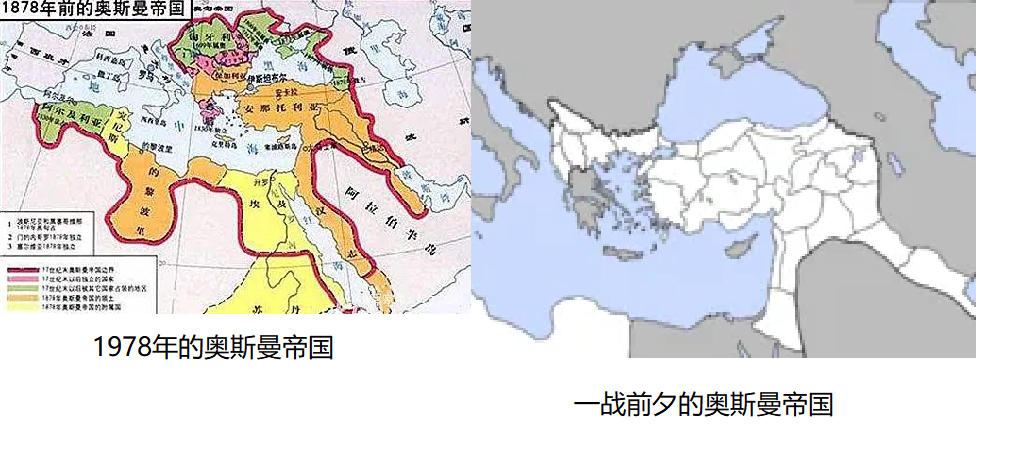
\includegraphics[width=6.4cm]{em.png}\\
\centering \zihao{5} Fig2.1 奥斯曼帝国19世纪末与一战前夕版图对比$^2$\footnotetext[2]{一战前夕意大利与奥斯曼帝国签署了《洛桑条约》,利比亚地区被其实际控制。利比亚也成为意大利在二战中的主要的殖民地}\clearpage
\justifying
于是,土耳其青年党准备寻找欧洲盟友,哪怕是一个欧洲强国的帮助,都可以让奥斯曼帝国抵御进一步侵略。奥斯曼帝国先找到了英国政府,英国外交部无情拒绝了它的结盟请求。1914年,他们又找到了另外三个欧洲列强:法、德、俄。亲法的奥斯曼海军大臣向法国示好,遭到了拒绝。曾经到过柏林的恩维尔向德国提交的提议又被德国大使拒绝。与俄国的结盟行动最终也遭到了拒绝。奥斯曼帝国遭到了彻底的外交孤立。

此时,英国人还没意识到奥斯曼帝国急切想要一个盟友,英国人还不知道,这直接导致了奥斯曼帝国在第一次世界大战中加入同盟国阵营对英作战。

1914年,欧洲的战争危机愈演愈烈。柏林方面开始重新考虑与奥斯曼帝国的关系。1914年7月24日,德皇威廉二世推翻了德国外交部拒绝与奥斯曼帝国合作的答复,重新考量与奥斯曼结盟的提议。就在前一天晚上,奥匈帝国向塞尔维亚发出了最后通牒,欧洲战争危机即将爆发。1914年8月1日,奥斯曼帝国正式与德国签署同盟协议。协议中包括了奥匈帝国最想要的“一旦奥斯曼帝国的领土遭遇威胁,德国有保卫其不受侵犯之义务,必要时应不惜诉诸武力。”。

1914年9月奥斯曼帝国发生了“戈本号”和“布雷斯劳号”事件,让英国开始感到奥斯曼帝国的敌意,但奥斯曼帝国仍没有对英宣战。1914年8月德军发动的坦能堡战役和9月的马祖里湖战役让俄国丢失大量土地,奥斯曼帝国意识到俄国即将输掉战争,如果再不参战,就再也没有机会分到俄国的土地。9月26日,青年土耳其党的军事大臣恩维尔在没有和其他人商量的情况下下令所有船只封锁达达尼尔海峡。这是恩维尔冲动的结果,他将所有筹码都押在了德国上,赌上了帝国的命运。恩维尔下令让“戈本号”和“布雷斯劳号”进入黑海袭击俄国船只。11月3日,英国战舰炮击了达达尼尔海峡要塞,标志着奥斯曼帝国与协约国的战争正式开始。

英国当时的海军大臣,也就是后来er
\clearpage
\end{document}